\chapter{Nasazení Foremanu}

Cílem této kapitoly je popsání nasazení frameworku Foreman, který jsme vybrali v~minulé kapitole. V~první části popíši topologii infrastruktury. Dále budou postupně popsány jednotilivé servery a služby, které na nich běží. Na konci kapitoly je popsán Ansible a jeho playbooky, pomocí kterých je možné infrastrukturu jednoduše nasadit.

\section{Topologie infrastruktury}

Jedním ze stavebních kamenů virtualizace je vymezení běhu operačního systému do virtualizovaného prostředí, přičemž jsou mu poskytnuty částečné či plné zdroje virtualizačním nástrojem. Díky tomu můžeme na jednom fyzickém stroji provozovat více virtuálních počítačů. Dává nám to možnost lépe a efektivněji využít výpočetního výkonu stroje (tzv. hypervisoru) s~dalšími výhodami, mezi které patří např. možnost hostování více operačních systémů na jednom serveru.
Výhodou virtualizovaných prostředí je dozajista oddělenost a jednoduché znovunasazení instancí. V~našem případě budeme jednotlivé části infrastuktury virtualizovat pomocí KVM.


\subsection{KVM}


KVM je virtualizační infrastruktura pro linuxové jádro, které ho přemění na hypervisor. Aplikaci začala vyvíjet společnost Qumranet, později odkoupená RedHatem. V~linuxovém kernelu je obsaženo od verze 2.6.20. Podporovaná je pouze plná virtualizace, plnou virtualizací ale lze spouštět i proprietární operační systémy, jako macOS, Windows, Solaris. Ke své funkčnosti vyžaduje nejméně podporu virtualizace procesoru první generace a to buď procesory od společnosti AMD pod označením AMD-VTM(1) či od společnosti Intel s~registrovanou ochranou známkou IntelR VT.



\begin{figure}[h]\centering
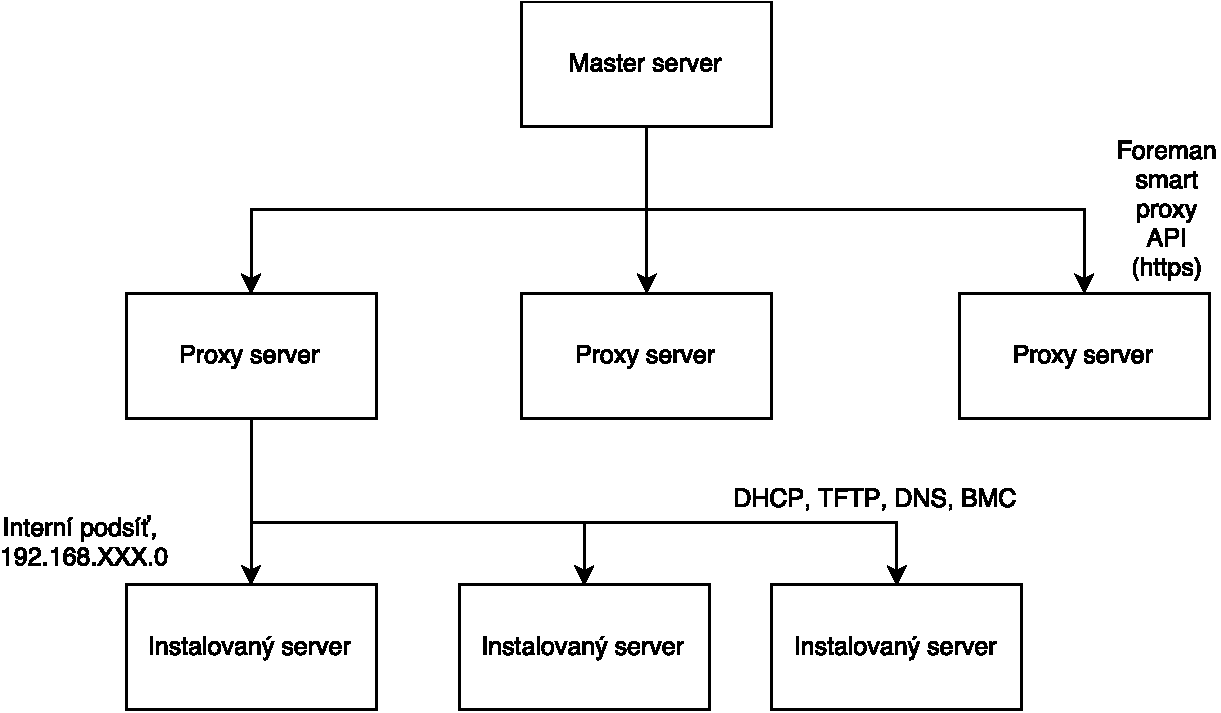
\includegraphics[width=1\textwidth]{files/infrastruktura-v2.pdf}
	\caption{Infrastruktura}\label{fig:float}
\end{figure}
